\chapter{White Matter Lesion Segmentation}
\label{sec:segmentation}

\section{Introduction}

\Gls{ms} is an inflammatory and demyelinating disease of the central nervous
system with pathology that can be observed in vivo by \gls{mri}.
MS is characterized by the formation of lesions, primarily visible in the white
matter on conventional MRI. Imaging biomarkers based on the delineation of
lesions, such as lesion load and lesion count, have established their importance
for assessing disease progression and treatment effect. However, lesions vary
greatly in size, shape, intensity and location, which makes their automatic and
accurate segmentation challenging.

\section[Related work]{Related Work}

Many automatic methods have been proposed for the segmentation of MS
\mbox{lesions} over the last two decades \citep{garcia2013}, which can be
classified into unsupervised and supervised methods.

\subsection[Unsupervised methods]{Unsupervised Methods}

Unsupervised methods do not require a labeled data set for training. Instead,
lesions are identified as an outlier of, e.g., a subject-specific generative
model of tissue intensities
\citep{vanleemput2001,tomas2015,schmidt2012,roura2015}, or a generative
model of image patches representing a healthy population \citep{weiss2013}.
Alternatively, clustering methods have been used to segment healthy and lesion
tissue, where lesions are modelled as a separate tissue class
\citep{shiee2010,sudre2015}. In many methods, spatial priors of healthy
tissues are used to reduce false positives. For example, in addition to
modelling MS lesions as a separate intensity cluster, Lesion-TOADS
\citep{shiee2010} employs topological and statistical atlases to produce
a topology-preserving segmentation of all brain tissues.

To account for local changes of the tissue intensity distributions,
\citet{tomas2015} combined the subject-specific model of
the global intensity distributions with a voxel-specific model calculated from a
healthy population, where lesions are detected as outliers of the combined
model. A major challenge of unsupervised methods is that outliers are often not
specific to lesions and can also be caused by intensity inhomogeneities, partial
volume, imaging artifacts, and small anatomical structures such as blood
vessels, which leads to the generation of false positives. To overcome these
limitations, \citet{roura2015} employed an additional set of rules
to remove false positives, while \citet{schmidt2012} used
a conservative threshold for the initial detection of lesions, which are later
grown in a separate step to yield an accurate delineation.

\subsection[Supervised methods]{Supervised Methods}

Current supervised approaches typically start with a set of features, which can
range from small and simple to large and highly variable, and are either
predefined by the user \citep{geremia2010,geremia2011,guizard2015,subbanna2015}
or gathered in a feature extraction step such as by deep learning \citep{yoo2014}.
Voxel-based segmentation algorithms \citep{geremia2010,yoo2014} feed the
features and labels of each voxel into a general classification algorithm, such
as a random forest \citep{breiman2001}, to classify each voxel and to determine
which set of features are the most important for segmentation in the particular
domain. Voxel features and the labels of neighboring voxels can be incorporated
into \glslink{mrf}{Markov random field-based (MRF-based)} approaches
\citep{subbanna2009,subbanna2015} to produce a spatially consistent
segmentation. As a strategy to reduce false positives, \citet{subbanna2015}
combined a voxel-level MRF with a regional MRF, which integrates a large
set of intensity and textural features extracted from the regions produced by the
voxel-level MRF with the labels of neighboring nodes of the regional MRF.
Library-based approaches leverage a library of pre-segmented images to carry out
the segmentation. For example, \citet{guizard2015} proposed a segmentation
method based on an extension of the non-local means algorithms
\citep{coupe2011}. The centres of patches at every voxel location are classified
based on matched patches from a library containing pre-segmented images, where
multiple matches are weighted using a similarity measure based on
rotation-invariant features.

\subsection[Patch-based deep learning methods]{Patch-based Deep Learning
Methods}

A recent breakthrough for the automatic image segmentation using deep learning
comes from the domain of cell membrane segmentation, in which
\citet{ciresan2012} proposed classifying the centres of image patches directly
using a \gls{cnn} \citep{lecun1998} without a dedicated feature extraction step.
Instead, features are learned indirectly within the lower layers of the neural
network during training, while the higher layers can be regarded as performing
the classification, which allows the learning of features that are specifically
tuned to the segmentation task. However, the time required to train patch-based
methods can make the approach infeasible when the size and number of patches are
large.

\subsection[Fully convolutional methods]{Fully Convolutional Methods}

Recently, different CNN architectures
\citep{li2014,long2015,ronneberger2015,brosch2015,kang2014} have been proposed
that are able to feed through entire images, which removes the need to select
representative patches, eliminates redundant calculations where patches overlap,
and therefore these models scale up more efficiently with image resolution.
\citet{kang2014} introduced the \gls{fcnn} for the segmentation of crowds
in surveillance videos. However, fCNNs produce segmentations of lower resolution
than the input images due to the successive use of convolutional and pooling
layers, both of which reduce the dimensionality. To predict segmentations of the
same resolution as the input images, we recently proposed using a 3-layer
\gls{cen} \citep{brosch2015} for MS lesion segmentation. The combination of
convolutional \citep{lecun1998} and deconvolutional \citep{zeiler2011} layers
allows our network to produce segmentations that are of the same resolution as
the input images.

Another limitation of the traditional CNN is the trade-off between localization
accuracy, represented by lower-level features, and contextual information,
provided by higher-level features. To overcome this limitation, \citet{long2015}
proposed fusing the segmentations produced by the lower layers of the network
with the upsampled segmentations produced by higher layers. However, using only
low-level features was not sufficient to produce a good segmentation at the
lowest layers, which is why segmentation fusion was only performed for the three
highest layers. Instead of combining the segmentations produced at different
layers, \citet{ronneberger2015} proposed combining the features of different
layers to calculate the final segmentation directly at the lowest layer using an
11-layer u-shaped network architecture called u-net. Their network is composed
of a traditional contracting path (first half of the u), but augmented with an
expanding path (last half of the u), which replaces the pooling layers of the
contracting path with upsampling operations. To leverage both high- and
low-level features, shortcut connections are added between corresponding layers
of the two paths. However, upsampling cannot fully compensate for the loss of
resolution, and special handling of the border regions is still required.

% We have evaluated our method on two widely used publicly available data sets for
% the evaluation of MS lesion segmentation methods and a large in-house data set
% from an MS clinical trial, with a comparison of network architectures of
% different depths and with and without shortcuts\footnote{Where the risk of
% confusion is minimal, we will refer to the shortcut connections between two
% corresponding layers as a single shortcut (see Fig. 1).}.

\section{Methods}
\label{sec:method}

We propose a new convolutional network architecture that combines the advantages
of a CEN \citep{brosch2015} and a u-net \citep{ronneberger2015}. Our network is
divided into two pathways, a traditional convolutional pathway, which consists
of alternating convolutional and pooling layers, and a deconvolutional pathway,
which consists of alternating deconvolutional and unpooling layers
\citep{zeiler2011} and predicts the final segmentation. Similar to the u-net, we
introduce shortcut connections between layers of the two pathways. In contrast
to the u-net, our method produces segmentations of the same resolution as the
input images, independent of the number of layers and filter sizes used, which
enables the use of deeper networks without requiring special handling of the
border regions.

\begin{figure*}[tb]
\centering
\begin{tikzpicture}[
  node distance=0.75cm and 0.65cm,
  font=\footnotesize,
  conv/.style={green!60!black,-latex,thick},
  conv2/.style={green!60!black,latex-latex,thick},
  deconv/.style={-latex,blue!40!black,thick},
  %pooling/.style={-latex,red!60!black,thick,dashed},
  %unpooling/.style={-latex,brown!60!black,thick,dashed},
  pooling/.style={-latex,green!60!black,thick,dashed},
  unpooling/.style={-latex,blue!40!black,thick,dashed},
  channel/.style args={#1 and #2}{draw, fill=lightgray, inner sep=0pt,
      minimum width=#1, minimum height=#2}
]

% \tikzstyle{channel}=[draw,minimum width=64pt,fill=lightgray,inner
% sep=0pt,minimum height=#1]

% Network

\begin{scope}[local bounding box=network]
\node[channel=64pt and 3pt,pin=270:Input images] (inputs) {};
\node[channel=60pt and 16pt,above=of inputs] (clayer1) {};
\node[channel=30pt and 16pt,above=of clayer1] (pooling1) {};

\node[channel=64pt and 1pt,right=of inputs,pin=270:Segmentations] (outputs) {};
\node[channel=60pt and 16pt] (dlayer1) at (clayer1-|outputs) {};
\node[channel=30pt and 16pt,above=of dlayer1] (dpooling1) {};

\node[fit=(pooling1)(dpooling1),inner sep = 0pt] (pooling) {};
\node[channel=26pt and 16pt,above=of pooling] (clayer2) {};
\end{scope}

\draw[conv] (inputs)--node[left] {$w^{(1)}_\text{c}$} (clayer1);
\draw[pooling] (clayer1)--node[left] {} (pooling1);
\draw[conv] (pooling1)--node[left] {$w^{(3)}_\text{c}$} (clayer2);
\draw[deconv] (clayer2)--node[right=5pt] {$w^{(3)}_\text{d}$} (dpooling1);
\draw[unpooling] (dpooling1)--node[right] {} (dlayer1);
\draw[deconv] (dlayer1)--node[right] {$w^{(1)}_\text{d}$} (outputs);
\draw[deconv] (clayer1)--node[anchor=188,inner sep=10pt]
{$w^{(1)}_\text{s}$}(outputs);

% Part labels

\node[left=1pt of inputs] {$x^{(0)}$};
\node[left=1pt of clayer1] {$x^{(1)}$};
\node[left=1pt of pooling1] {$x^{(2)}$};
\node[left=1pt of clayer2] {$x^{(3)}$};

\node[right=1pt of outputs] {$y^{(0)}$};
\node[right=1pt of dlayer1] {$y^{(1)}$};
\node[right=1pt of dpooling1] {$y^{(2)}$};
\node[right=1pt of clayer2] {$y^{(3)}$};

% Layers

\draw[decorate,decoration={brace,raise=30pt}] (inputs.south west)
--node[left=35pt,align=center] (convl) {Convolutional\\ layer} (inputs.south
west|-clayer1.north west);

\draw[decorate,decoration={brace,raise=22pt}] (clayer1.south west)
--node[left=27pt,align=center] {Pooling\\ layer} (clayer1.south
west|-pooling1.north west);

\draw[decorate,decoration={brace,raise=25pt}] (pooling1.south west)
--node[left=30pt,align=center] {Convolutional\\ layer} (clayer2.north
west-|pooling1.south west);

\draw[decorate,decoration={brace,raise=30pt,mirror}] (outputs.south east)
--node[right=35pt,align=center] {Deconvolutional\\ layer with shortcut}
 (dlayer1.north east-|outputs.south east);

\draw[decorate,decoration={brace,raise=22pt,mirror}] (dlayer1.south east)
--node[right=27pt,align=center] {Unpooling\\ layer}
(dpooling1.north east-|dlayer1.south east);

\draw[decorate,decoration={brace,raise=25pt,mirror}] (dpooling1.south east)
--node[right=30pt,align=center] {Deconvolutional\\ layer}
(clayer2.north east-|dpooling1.south east);

% Legend

\begin{scope}[local bounding box=ghost,opacity=0]
\path[conv] node (conv) {convolution} [draw] (conv.west)
++(left:0.5)--++(right:0.5);

\path[pooling] node[right=0.8 of conv] (pool) {pooling} [draw] (pool.west)
++(left:0.5)--++(right:0.5);

\path[deconv] node[right=0.8 of pool] (dconv) {deconvolution} [draw]
(dconv.west) ++(left:0.5)--++(right:0.5);

\path[unpooling] node[right=0.8 of dconv] (unpool) {unpooling} [draw]
(unpool.west) ++(left:0.5)--++(right:0.5);
\end{scope}

\begin{scope}[local bounding box=ghost2,
    shift={($(network.south)-(ghost.north)$)},xshift=2pt,yshift=-7pt]

\path[conv] node (conv) {convolution} [draw] (conv.west)
++(left:0.5)--++(right:0.5);

\path[pooling] node[right=0.8 of conv] (pool) {pooling} [draw] (pool.west)
++(left:0.5)--++(right:0.5);

\path[deconv] node[right=0.8 of pool] (dconv) {deconvolution} [draw]
(dconv.west) ++(left:0.5)--++(right:0.5);

\path[unpooling] node[right=0.8 of dconv] (unpool) {unpooling} [draw]
(unpool.west) ++(left:0.5)--++(right:0.5);
\end{scope}

% Stack of CRBMs

\begin{scope}[local bounding box=dbn]
\node[channel=64pt and 3pt, left=6cm of inputs,pin=270:Input images] (rinputs)
{}; 
\node[channel=60pt and 16pt,above=of rinputs] (rclayer1) {};
\node[channel=30pt and 16pt,above=of rclayer1] (rpooling1) {};
\node[channel=26pt and 16pt,above=of rpooling1] (rclayer2) {};
\end{scope}

\draw[conv2] (rinputs)--node[left] {$\hat{w}^{(1)}$} (rclayer1);
\draw[pooling] (rclayer1)--node[right] {pooling} (rpooling1);
\draw[conv2] (rpooling1)--node[left] {$\hat{w}^{(2)}$} (rclayer2);

\node[left=1pt of rinputs] {$v^{(1)}$};
\node[left=1pt of rclayer1] {$h^{(1)}$};
\node[left=1pt of rpooling1] {$v^{(2)}$};
\node[left=1pt of rclayer2] {$h^{(2)}$};

\draw[decorate,decoration={brace,raise=5pt,mirror}] (rinputs.south east)
--node[right=10pt,align=center] (crbm) {convRBM$_1$} (rinputs.south
east|-rclayer1.north east);

\draw[decorate,decoration={brace,raise=5pt,mirror}] (rpooling1.south east)
--node[right=10pt,align=center] {convRBM$_2$} (rclayer2.north
east-|rpooling1.south east);

% \node[above=10pt of dbn,align=center] {Stack of Convolutional\\ Restricted
% Boltzmann Machines};
% \node[above=10pt of network] {Convolutional Encoder Network};

\node[above=15pt of dbn,align=center,font=\normalsize] {Pre-training};
\node[above=15pt of network,font=\normalsize] {Fine-tuning};

% \draw[->] (crbm.east|-dbn)-- node[above=2pt] {convert} 
% node[above,align=center]
% {$w_\text{c}^{(1)} = w^{(1)}$ \\
%  $w_\text{c}^{(2)} = w^{(2)}$ \\
%  $w_\text{d}^{(2)} = w^{(2)}$ \\
%  $w_\text{d}^{(1)} = 0.5w^{(1)}$ \\
%  $w_\text{s}^{(1)} = 0.5w^{(1)}$}
% (convl.west|-network);

%\draw (network.north west) rectangle (network.south east);
%\draw (ghost.north west) rectangle (ghost.south east);
%\draw (ghost2.north west) rectangle (ghost2.south east);

%\path[pooling] node (pool) at (-3,-1) {convolution};
%\draw[pooling] (conv.west) ++(left:0.5)--++(right:0.5);

%\draw[conv] (-3,-1)-- +(right:0.5) node[right] {convolution};
%\draw[pooling] (-0.5,-1)-- +(right:0.5) node[right] {pooling};
%\draw[deconv] (2,-1)-- +(right:0.5) node[right] {deconvolution};
%\draw[unpooling] (4.5,-1)-- +(right:0.5) node[right] {unpooling};

%\draw[pooling] (0,-1.5)-- +(right:0.5) node[right] {pooling};
%\draw[deconv] (0,-2)-- +(right:0.5) node[right] {deconvolution};
%\draw[unpooling] (0,-2.5)-- +(right:0.5) node[right] {unpooling};

\end{tikzpicture}

\caption[Pre-training and fine-tuning a 7-layer convolutional encoder network
with shortcut]{Pre-training and fine-tuning a 7-layer convolutional encoder
network with shortcut. The activations calculated by deconvolution through a
shortcut are added to the corresponding layer activations before applying the
transfer function. For deeper network architectures, there is a shortcut
between all convolutional and deconvolutional layers except for the top-most
layer. Pre-training is performed on the input images using a stack of
convolutional RBMs. The pre-trained weights and bias terms are used to
initialize a CEN, which is fine-tuned on pairs of input images, $x^{(0)}$, and
segmentations, $y^{(0)}$.}

\label{fig:network}
\end{figure*}

% \subsection[Segmentation as an optimization problem]{Segmentation as an
% Optimization Problem}

The task of segmenting MS lesions is defined as finding a function $s$ that maps
multi-modal images $I$, e.g., $I = (I_\text{FLAIR}, I_\text{T1})$, to
corresponding binary lesion masks $S$, where $1$ denotes a lesion voxel and $0$
denotes a non-lesion voxel. Given a set of training images $I_n$, $n \in \N$,
and corresponding segmentations $S_n$, we model finding an appropriate function
for segmenting MS lesions as an optimization problem of the following form
\begin{equation}
\hat{s} = \arg \min_{s \in \mathcal{S}} \sum_n E(S_n, s(I_n)),
\label{eq:segprob}
\end{equation}
where $\mathcal{S}$ is the set of possible segmentation functions, and $E$ is an
error measure that calculates the dissimilarity between ground truth
segmentations and predicted segmentations. The set of possible segmentation
functions $\mathcal{S}$ is defined by the network architecture, where a
particular function $s$ is defined by the combination of network architecture
and learned parameters of the network.

\subsection[Model architecture]{Model Architecture}

The set of possible segmentation functions, $\mathcal{S}$, is modelled by the
\gls{cens} illustrated in \ref{fig:network}. A CEN-s is a type of \gls{cnn}
\citep{lecun1998} that is divided into two interconnected pathways, the
convolutional pathway and the deconvolutional \citep{zeiler2011} pathway. The
convolutional pathway consists of alternating convolutional and pooling layers.
The input layer of the convolutional pathway is composed of the image voxels
$x^{(0)}_i(\vect{p})$, $i \in [1, C]$, where $i$ indexes the modality or input
channel, $C$ is the number of modalities or channels, and $\vect{p} \in \N^3$
are the coordinates of a particular voxel. The convolutional layers
automatically learn a feature hierarchy from the input images. A convolutional
layer is a deterministic function of the following form
\begin{equation}
x^{(l)}_j = \max \Bigg(0, \sum_{i=1}^C\tilde{w}^{(l)}_{\text{c},ij}*x^{(l-1)}_i
+ b^{(l)}_j\Bigg),
\end{equation}
where $l$ is the index of a convolutional layer, $x^{(l)}_j$, $j \in [1,F]$,
denotes the feature map corresponding to the trainable convolution filter
$w^{(l)}_{\text{c},ij}$, $F$ is the number of filters of the current layer,
$b^{(l)}_j$ are trainable bias terms, $*$ denotes valid convolution, and
$\tilde{w}$ denotes a flipped version of $w$, i.e., $\tilde{w}(a) = w(-a)$. To
be consistent with the inference rules of \glspl{crbm}
\citep{lee2009}, which are used for pre-training, convolutional
layers convolve the input signal with flipped filter kernels, while
deconvolutional layers calculate convolutions with non-flipped filter kernels.
We use rectified linear units \citep{nair2010} in all layers except for the
output layers, which have shown to improve the classification performance of
CNNs \citep{krizhevsky2012}. A convolutional layer is followed by an average
pooling layer \citep{scherer2010} that halves the number of units in
each dimension by calculating the average of each block of \num{2x2x2} units per
channel.

The deconvolutional pathway consists of alternating deconvolutional and
unpooling layers with shortcut connections to the corresponding
convolutional layers. The first deconvolutional layer uses the extracted
features of the convolutional pathway to calculate abstract segmentation
features
\begin{equation}
y^{(L-1)}_i = \max\Bigg(0, \sum_{j=1}^Fw^{(L)}_{\text{d},ij}\circledast
y^{(L)}_j + c^{(L-1)}_{i}\Bigg),
\end{equation}
where $y^{(L)} = x^{(L)}$, $L$ denotes the number of layers of the convolutional
pathway, $w^{(L)}_{\text{d},ij}$ and $c^{(L-1)}_i$ are trainable parameters of
the deconvolutional layer, and $\circledast$ denotes full convolution. To be
consistent with the general notation of deconvolutions \citep{zeiler2011}, the
non-flipped version of $w$ is convolved with the input signal.

Subsequent deconvolutional layers use the activations of the previous layer and
corresponding convolutional layer to calculate more localized segmentation
features
\begin{equation}
y^{(l)}_i = \max\Bigg(0, 
\sum_{j=1}^Fw^{(l+1)}_{\text{d},ij}\circledast y^{(l+1)}_j
+ \sum_{j=1}^F w^{(l+1)}_{\text{s},ij}\circledast x^{(l+1)}_j +
c^{(l)}_i\Bigg),
\end{equation}
where $l$ is the index of a deconvolutional layer with shortcut, and
$w^{(l+1)}_{\text{s},ij}$ are the shortcut filter kernels connecting the
activations of the convolutional pathway with the activations of the
deconvolutional pathway. The last deconvolutional layer integrates the low-level
features extracted by the first convolutional layer with the high-level features
from the previous layer to calculate a probabilistic lesion mask
\begin{equation}
y^{(0)}_1 = \sigm\Bigg(\sum_{j=1}^F\Big(w^{(1)}_{\text{d},1j}\circledast
y^{(1)}_j +
w^{(1)}_{\text{s},1j}\circledast x^{(1)}_j\Big) + c^{(0)}_1\Bigg),
\end{equation}
where we use the sigmoid function defined as $\sigm(z) = (1 + \exp(-z))^{-1}, z
\in \R$, instead of the rectified linear function in order to obtain a
probabilistic segmentation with values in the range between 0 and 1.
To produce a binary lesion mask from the probabilistic output of our model, we
chose a fixed threshold such that the mean \gls{dsc} \citep{dice1945measures}
is maximized on the training set and used the same threshold for the evaluation
on the test set.

\subsection[Gradient calculation]{Gradient Calculation}

The parameters of the model can be efficiently learned by minimizing the error
$E$ for each sample of the training set, which requires the calculation of the
gradient of $E$ with respect to the model parameters \citep{lecun1998}.
Typically, neural networks are trained by minimizing either the \gls{ssd} or the
cross-entropy. Here, we will derive the gradient on the example of the
\gls{ssd}, due to the similarity of the \gls{ssd} with the later proposed
objective function. The \gls{ssd} can be calculated for a single image as
follows
\begin{equation}
% Error function
E = \frac{1}{2}\sum_{\vect{p}}\left(S(\vect{p}) -
y^{(0)}(\vect{p})\right)^2,
\end{equation}
where $\vect{p} \in \N^3$ are the coordinates of a particular voxel.
The partial derivatives of the error with respect to the model parameters can be
calculated using the delta rule and are given by 
\begin{align}
\label{eq:dEd}
% Deconvolutional filters
\frac{\partial E}{\partial w^{(l)}_{\text{d},ij}} &=
\delta^{(l-1)}_{\text{d},i} * \tilde{y}^{(l)}_j, &
% Deconvolutional bias
\frac{\partial E}{\partial c^{(l)}_i} &= \sum_{\vect{p}}
\delta^{(l)}_{\text{d},i}(\vect{p}), \\
\label{eq:dEs}
% Shortcut filters
\frac{\partial E}{\partial w^{(l)}_{\text{s},ij}}
 &= \delta^{(l-1)}_{\text{d},i} * \tilde{x}^{(l)}_j, \\
 \label{eq:dEc}
% Convolutional filters
\frac{\partial E}{\partial w^{(l)}_{\text{c},ij}} 
&= x^{(l-1)}_i * \tilde{\delta}^{(l)}_{\text{c},j},\text{ and}&
% Convolutional bias
\frac{\partial E}{\partial b^{(l)}_i} &= \sum_{\vect{p}}
\delta^{(l)}_{\text{c},i}(\vect{p}).
\end{align}
For the output layer, $\delta^{(0)}_{\text{d},1}$ can be calculated by
\begin{equation}
% Delta update
\delta^{(0)}_{\text{d},1} = \big(y^{(0)}_1
-S\big)y^{(0)}_1\big(1-y^{(0)}_1\big).
\label{eq:delta0}
\end{equation}
The derivatives of the error with respect to the parameters of the other layers
can be calculated by applying the chain rule of partial derivatives, which
yields to
\begin{align}
\label{eq:deltad}
% Delta update of deconvolutional layer
\delta^{(l)}_{\text{d},j} &= \sum_i^C
\big(\tilde{w}^{(l)}_{\text{d},ij}*\delta^{(l-1)}_{\text{d},i}\big)\I\big(y^{(l)}_j
> 0\big),\\
\label{eq:deltac}
% Delta update of convolutional layer
\delta^{(l)}_{\text{c},i} &= \sum_j^F
\big(w^{(l+1)}_{\text{c},ij}\circledast\delta^{(l+1)}_{\text{c},j}\big)\I\big(x^{(l)}_i
> 0\big),
\end{align}
where $l$ is the index of a deconvolutional or convolutional layer,
$\delta^{(L)}_{\text{c},i} = \delta^{(L)}_{\text{d},j}$, and $\I(z)$ denotes the
indicator function defined as $1$ if the predicate $z$ is true and $0$
otherwise. If a layer is connected through a shortcut,
$\delta^{(l)}_{\text{c},j}$ needs to be adjusted by propagating the error back
through the shortcut connection. In this case, $\delta^{(l)}_{\text{c},j}$ is
calculated by
\begin{equation}
% Delta update convolutional with shortcut
\delta^{(l)}_{\text{c},j} =
\big(\delta^{(l)}_{\text{c},j}{}'+
\tilde{w}^{(l)}_{\text{s},ij}*\delta^{(l-1)}_{\text{d},i}\big)\I\big(x^{(l)}_j
> 0\big),
\label{eq:deltas}
\end{equation}
where $\delta^{(l)}_{\text{c},j}{}'$ denotes the activation of unit
$\delta^{(l)}_{\text{c},j}$ before taking the shortcut connection into account.

The sum of squared differences is a good measure of classification accuracy, if
the two classes are fairly balanced. However, if one class contains vastly more
samples, as is the case for lesion segmentation, the error measure is dominated
by the majority class and consequently, the neural network would learn to ignore
the minority class. To overcome this problem, we use a combination of
sensitivity and specificity, which can be used together to measure
classification performance even for vastly unbalanced problems. More precisely,
the final error measure is a weighted sum of the mean squared difference of the
lesion voxels (sensitivity) and non-lesion voxels (specificity), reformulated to
be error terms:
\begin{equation} 
E = r\frac{\textstyle\sum_{\vect{p}} \left(S(\vect{p}) -
y^{(0)}(\vect{p})\right)^2 S(\vect{p})}{\textstyle\sum_{\vect{p}} S(\vect{p})}
 + (1-r)\frac{\textstyle\sum_{\vect{p}} \left(S(\vect{p}) -
y^{(0)}(\vect{p})\right)^2 \big(1 - S(\vect{p})\big)}{%
\textstyle\sum_{\vect{p}}\big(1 - S(\vect{p})\big)}.
\end{equation}
We formulate the sensitivity and specificity errors as squared errors in order
to yield smooth gradients, which makes the optimization more robust. The
sensitivity ratio $r$ can be used to assign different weights to the two terms.
Due to the large number of non-lesion voxels, weighting the specificity error
higher is important, but based on preliminary experimental results
\citep{brosch2015}, the algorithm is stable with respect to changes in $r$,
which largely affects the threshold used to binarize the probabilistic output. A
detailed evaluation of the impact of the sensitivity ratio on the learned model
is presented in \ref{sec:trainparams}.

To train our model, we must compute the derivatives of the modified objective
function with respect to the model parameters. Equations
\ref{eq:dEd}--\ref{eq:dEc} and \ref{eq:deltad}--\ref{eq:deltas} are a
consequence of the chain rule and independent of the chosen similarity measure.
Hence, we only need to derive the update rule for $\delta^{(0)}_{\text{d},1}$.
With $\alpha = 2r (\sum_{\vect{p}}S(\vect{p}))^{-1}$ and $\beta = 2(1 -
r)(\sum_{\vect{p}}(1 - S(\vect{p})))^{-1}$, we can rewrite $E$ as
\begin{align}
E=& \frac{1}{2}\sum_{\vect{p}}\left(S(\vect{p}) - y^{(0)}(\vect{p})\right)^2
\alpha S(\vect{p}) +
\frac{1}{2}\sum_{\vect{p}}\left(S(\vect{p})-y^{(0)}(\vect{p})\right)^2
\beta\big(1-S(\vect{p})\big)\\
=& \frac{1}{2}\sum_{\vect{p}}\big(\alpha S(\vect{p}) +
\beta(1-S(\vect{p}))\big)\Big(S(\vect{p})-y^{(0)}_1(\vect{p})\Big)^2.
\end{align}
Our objective function is similar to the SSD, with an additional multiplicative
term applied to the squared differences. The additional factor only depends on
the target segmentation $S$ and is therefore constant with
respect to the model parameters. Consequently, $\delta^{(0)}_{\text{d},1}$ can
be derived analogously to the SSD case, and the new factor is simply carried
over:
\begin{equation} 
\delta^{(0)}_{\text{d},1} = \big(\alpha S + \beta (1 - S)\big)\big(y^{(0)}_1 -
S\big) y^{(0)}_1 \big(1 - y^{(0)}_1\big).
\end{equation}

\subsection{Training}

At the beginning of the training procedure, the model parameters need to be
initialized and the choice of the initial parameters can have a big impact on
the learned model \citep{sutskever2013}. In our experiments, we found
that initializing the model using pre-training \citep{hinton2006c} on the input
images was required in order to be able to fine-tune the model using the ground
truth segmentations without getting stuck early in a local minimum. Pre-training
can be performed layer by layer \citep{hinton2006b} using a stack of convRBMs
(see \ref{fig:network}), thereby avoiding the potential problem of
vanishing or exploding gradients \citep{hochreiter1991untersuchungen}. The first
convRBM is trained on the input images, while subsequent convRBMs are trained on
the hidden activations of the previous convRBM. After all convRBMs have been
trained, the model parameters of the CEN-s can be initialized as follows
(showing the first convolutional and the last deconvolutional layers only, see
\ref{fig:network})

\begin{align}
w_{\text{c}}^{(1)} &= \hat{w}^{(1)}, &
w_{\text{d}}^{(1)} &= 0.5\hat{w}^{(1)}, &
w_{\text{s}}^{(1)} &= 0.5\hat{w}^{(1)} \\
b^{(1)} &= \hat{b}^{(1)}, &
c^{(0)} &= \hat{c}^{(1)},
\end{align}
where $\hat{w}^{(1)}$ are the filter weights, $\hat{b}^{(1)}$ are the hidden
bias terms, and $\hat{c}^{(1)}$ are the visible bias terms of the first convRBM.

A major challenge for gradient-based optimization methods is the choice of an
appropriate learning rate. Classic stochastic gradient descent \citep{lecun1998}
uses a fixed or decaying learning rate, which is the same for all parameters of
the model. However, the partial derivatives of parameters of different layers
can vary substantially in magnitude, which can require different learning rates.
In recent years, there has been an increasing interest in developing methods for
automatically choosing independent learning rates. Most methods (e.g., AdaGrad
by \citealp{duchi2011}; AdaDelta by \citealp{zeiler2012};
RMSprop by \citealp{dauphin2015}; and Adam by \citealp{kingma2014})
collect different statistics of the partial derivatives over multiple iterations
and use this information to set an adaptive learning rate for each parameter.
This is especially important for the training of deep networks, where the
optimal learning rates often differ greatly for each layer. In our initial
experiments, networks obtained by training with AdaDelta, RMSprop, and Adam
performed comparably well, but AdaDelta was the most robust to the choice of
hyperparameters, so we used AdaDelta for all results reported.

\subsection{Implementation}

Pre-training and fine-tuning were performed using the highly optimized
GPU-accelerated implementation of 3D convRBMs and CNNs
\citep{brosch2015efficient} explained in \ref{sec:training}. Our frequency
domain implementation significantly speeds up the training by mapping the
calculation of convolutions to simple element-wise multiplications, while adding
only a small number of Fourier transforms. This is especially beneficial for the
training on 3D volumes, due to the increased number of weights of 3D kernels
compared to 2D. Although GPU-accelerated deep learning libraries based on the
\gls{cudnn} \citep{chetlur2014} are publicly available (e.g.,
\citealp{jia2014,bastien2012,collobert2011torch7}), we trained our models using
our own implementation, because we optimized it for memory facilitating the
training on large 3D volumes and because it performs the most computationally
intensive training operations six times faster than cuDNN in a direct comparison
(see \ref{tab:usedmodels} on page \pageref{tab:usedmodels}).
 
\sisetup{separate-uncertainty=true,detect-weight=true,detect-inline-weight=math}

\section[Experiments and results]{Experiments and Results}

We evaluated our method on two publicly available data sets (from the MICCAI
2008 MS lesion segmentation
challenge\footnote{\url{http://www.ia.unc.edu/MSseg/}} and the ISBI 2015
longitudinal MS lesion segmentation
challenge\footnote{\url{http://iacl.ece.jhu.edu/MSChallenge}}), which allows for
a direct comparison with many state-of-the-art methods. In addition, we have
used two much larger data sets containing two and four different MRI sequences
from a multi-centre clinical trial in secondary progressive MS and relapsing
remitting MS, which tends to have the most heterogeneity among the MS subtypes.
These data sets are challenging due to the large variability in lesion size,
shape, location, and intensity as well as varying contrasts produced by
different scanners. The clinical trial data sets were used to estimate the
number of images required to train a CEN without overfitting and to carry out a
detailed analysis of different CEN architectures using different combinations of
modalities, with a comparison to five publicly available state-of-the-art
methods.

\subsection[Data sets and preprocessing]{Data Sets and Preprocessing}

\subsubsection{Public Data Sets}
The data set of the MICCAI 2008 MS lesion segmentation challenge
\citep{styner20083d} consists of 43 \gls{t1w}, \gls{t2w}, and
\gls{flair} MRIs, divided into 20 training cases for which ground truth
segmentations are made publicly available, and 23 test cases. In a first
experiment, we evaluated our method on the 20 training cases using 5-fold
cross-validation. In a second experiment, we trained our model on the 20
training cases and then used the trained model to segment the 23 test cases,
which were sent to the challenge organizers for independent evaluation.

The data set of the ISBI 2015 longitudinal MS lesion segmentation challenge
consists of 21 visit sets, each with T1w, T2w, \gls{pdw}, and FLAIR MRIs. The
challenge was not open for new submissions at the time of writing this article.
Therefore, we evaluated our method on the training set using
leave-one-subject-out cross-validation, following the evaluation protocol of the
second place method by \citet{jesson2015} and third place method by
\citet{maier2015} from the challenge proceedings. The paper of the first place
method does not have sufficient details to replicate their evaluation.

\subsubsection{Clinical Trial Data Sets}

%TODO: Please add more details about the source of the
% two datasets and the characteristics of the data (population characteristics,
% disease prevalence, scanners, etc).

We used two different clinical trial data sets to evaluate our method. The first
data set contains images of 500 subjects split equally into training and test
sets. The images were acquired from 45 different scanning sites. For each
subject, the data set contains T2- and PD-weighted MRIs with a voxel size of
\SI{0.937x0.937x3.000}{\milli\metre}. The main preprocessing steps included
rigid intra-subject registration, brain extraction, intensity normalization, and
background cropping. This data set was used to evaluate how many images are
required to train a simple 3-layer CEN without overfitting. Training on a
single GeForce GTX 780 graphics card took between 6 and 32 hours per model
depending on the training set size. However, once the network is trained,
segmentation of new images can be performed in less than one second.

The second data set was collected from 67 different scanning sites using
different 1.5\,T and 3\,T scanners, and consists of T1w, T2w, PDw, and FLAIR
MRIs from 195 subjects, most with two time points (377 visit sets in total). In
contrast to the previous data set, this data set also contains T1w and FLAIR
MRIs, which allows for a direct comparison with other competing methods, which
require these modalities. The image dimensions and voxel sizes vary by site, but
most of the T1w images have close to \SI{1}{\milli\meter} isotropic voxels,
while the other images have voxel sizes close to \SI{1x1x3}{\milli\meter}. All
images were skull-stripped using the brain extraction tool (BET)
\citep{jenkinson2005}, followed by an intensity normalization to the
interval $[0,1]$, and a 6 degree-of-freedom intra-subject registration using one
of the \SI{3}{\milli\meter} scans as the target image to align the different
modalities. To speed-up the training, all images were cropped to a
\num{164x206x52} voxel subvolume with the brain roughly centred. The ground
truth segmentations for both data sets were produced using an existing
semiautomatic 2D region-growing technique, which has been used successfully in a
number of large MS clinical trials (e.g.,
\citealp{kappos2006,traboulsee2008}).
Each lesion was manually identified by an experienced radiologist and then
interactively grown from the seed point by a trained technician.

We divided the data set into a training ($n=250$), validation ($n=50$), and test
set ($n=77$) such that images of each set were acquired from different scanning
sites. The training, validation, and test sets were used for training our
models, for monitoring the training progress, and to evaluate performance,
respectively. The training set was also used to perform parameter tuning of the
other methods used for comparison. Pre-training and fine-tuning of our 7-layer
CEN-s took approximately 27 hours and 37 hours, respectively, on a single
GeForce GTX 780 graphics card. Once the network is trained, new multi-contrast
images can be segmented in less than one second.

\subsection[Comparison to other methods]{Comparison to Other Methods}
\label{sec:othermethods}

We compared our method with five publicly available methods, some of which
are widely used for clinical research and are established in the literature
(e.g., \citealp{sudre2015,subbanna2015,guizard2015}) as reference points for
comparison. These five methods include:
\begin{enumerate}
\item \Gls{ems} method \citep{vanleemput2001};
\item \Gls{lga} \citep{schmidt2012}, as
implemented in the \gls{lst} version 2.0.11;
\item \Gls{lpa} also implemented in the same LST toolbox;
\item Lesion-TOADS version 1.9 R \citep{shiee2010}; and 
\item \Gls{sls} toolbox \citep{roura2015}.
\end{enumerate}
The Lesion-TOADS software only takes T1w and FLAIR MRIs and has no tunable
parameters, so we used the default parameters to carry out the segmentations.
The performance of EMS depends on the choice of the Mahalanobis distance
$\kappa$, the threshold $t$ used to binarize the probabilistic segmentation, and
the modalities used. We applied EMS to segment lesions using two combinations of
modalities: a) T1w, T2w, and PDw, as used in the original paper
\citep{vanleemput2001}, and b) all four available modalities (T1w, T2w, PD2,
FLAIR). We compared the segmentations produced for all combinations of $\kappa =
2.0, 2.2, \dotsc, 4.6$ and $t = 0.05, 0.10, \dotsc, 1.00$ with the ground truth
segmentations on the training set and chose the values that maximized the
average DSC ($\kappa = 2.6, t = 0.75$ for three modalities; $\kappa = 2.8, t =
0.9$ for four modalities).

The LST-LGA and LST-LPA of the LST toolbox only take T1w and FLAIR MRIs as
input, and we used those modalities to tune the initial threshold $\kappa$ of
LST-LGA for $\kappa = 0.05, 0.10, \dotsc, 1.00$ and the threshold $t$ used by
LST-LPA to binarize the probabilistic segmentations for $t = 0.05, 0.10, \dotsc,
1.00$. The optimal parameters were $\kappa = 0.10$ and $t = 0.45$, respectively.

Similarly, the SLS toolbox, which is the most recently published work
\citep{roura2015} also only takes T1w and FLAIR MRIs as input. This method uses
an initial brain tissue segmentation obtained from the T1w images and segments
lesions by treating lesional pixels as outliers to the normal appearing grey
matter brain tissue on the FLAIR images. This method has three key parameters:
$\omega_\text{nb}$, $\omega_\text{ts}$, and $\alpha_\text{sls}$. We tuned these
parameters on the training set via a grid-search over a range of values as
suggested by \citet{roura2015}.

\subsection[Measures of segmentation accuracy]{Measures of Segmentation
Accuracy}
 
We used the following six measures to produce a comprehensive evaluation
of segmentation accuracy as there is generally no single measure that is
sufficient to capture all information relevant to the quality of a produced
segmentation \citep{garcia2013}.

The first measure is the \gls{dsc}
\citep{dice1945measures} that computes a normalized overlap value between the
produced and ground truth segmentations, and is defined as
\begin{equation}
\text{DSC} = \frac{2 \times \text{TP}}{2 \times \text{TP} + \text{FP} +
\text{FN}},
\end{equation}
\glsunset{tp}\glsunset{fp}\glsunset{fn}%
where \gls{tp}, \gls{fp}, and \gls{fn} denote the number of true positive, false
positive, and false negative voxels, respectively. A value of \SI{100}{\percent}
indicates a perfect overlap of the produced segmentation and the ground truth.
The DSC incorporates measures of over- and underestimation into a single metric,
which makes it a suitable measure to compare overall segmentation accuracy. In
addition, we have used the \gls{tpr} and the \gls{ppv} to provide further
information on specific aspects of segmentation performance. The TPR is used to measure the fraction of the lesion regions in
the ground truth that are correctly identified by an automatic method. It is
defined as
\begin{equation}
\text{TPR} = \frac{\text{TP}}{\text{TP} + \text{FN}},
\end{equation}
where a value of \SI{100}{\percent} indicates that all true lesion voxels are
correctly identified. The PPV is used to determine the extent of
the regions falsely classified as lesion by an automatic method.
It is defined as the fraction of true lesion voxels out of all
identified lesion voxels
\begin{equation}
\text{PPV} = \frac{\text{TP}}{\text{TP} + \text{FP}},
\end{equation}
where a value of \SI{100}{\percent} indicates that all voxels that are
classified as lesion voxels are indeed lesion voxels as defined by the ground
truth (no false positives).

We also measured the \gls{vd} between the ground truth and the produced
segmentation by computing their volumes (Vol), i.e.,
\begin{equation}
\text{VD} = \frac{\text{Vol}(\text{Seg}) - \text{Vol}(\text{GT})}
                {\text{Vol}(\text{GT})},
\end{equation}
where Seg and GT denote the obtained segmentation and ground truth,
respectively. However, it has been noted \citep{garcia2013} that a wide
variability exists even between the lesion segmentations of trained experts, and
thus, the achieved volume differences reported in the literature have ranged
from \SI{10}{\percent} to \SI{68}{\percent}.

For more precise evaluation, we have also included the \gls{ltpr} and the
\gls{lfpr} that are much more sensitive in measuring the segmentation accuracy
of smaller lesions, which are important to detect when performing early disease
diagnosis \citep{garcia2013}. More specifically, the LTPR measures the TPR
on a per lesion-basis and is defined as
\begin{equation}
\text{LTPR} = \frac{\text{LTP}}{\text{\#RL}},
\end{equation}
where LTP denotes the number of lesion true positives, i.e., the number
lesions in the reference segmentation that overlap with a lesion in the produced
segmentation, and \#RL denotes the total number of lesions in the reference
segmentation. An LTPR with a value of \SI{100}{\percent} indicates that all
lesions are correctly identified. Similarly, the lesion-wise false positive rate
(FPR) measures the fraction of the segmented lesions that are not in the ground
truth and is defined as
\begin{equation}
\text{LFPR} = \frac{\text{LFP}}{\text{\#PL}},
\end{equation}
where LFP denotes the number of lesion false positives, i.e., the number of
lesions in the produced segmentation that do not overlap with a lesion in the
reference segmentation, and \#PL denotes the total number of lesions in the
produced segmentation. An LFPR with a value of \SI{0}{\percent} indicates that
no lesions were incorrectly identified.

\subsection[Training parameters]{Training Parameters}
\label{sec:trainparams}

In this set of experiments, we evaluated the impact of the number of epochs and
the sensitivity ratio on the trained networks. \ref{fig:epochs} shows the mean
DSC evaluated on the training and validation sets of the second clinical data
set as computed during training of a \mbox{7-layer} CEN-s up to 500 epochs. The
mean DSC scores increase monotonically, but the improvements are minor after 400
epochs. The optimal number of epochs is a trade-off between accuracy and time
required for training.
Due to the relatively small improvements after 400 epochs, we decided to stop
the training procedure at 500 epochs. For the challenge data sets, due to their
small sizes, we did not employ a subset of the data for a dedicated validation
set to choose the number of epochs. Instead, we set the number of epochs to
2500, which corresponds to roughly the same number of gradient updates compared
to the clinical trial data set.

\begin{figure}[tb]
\centering
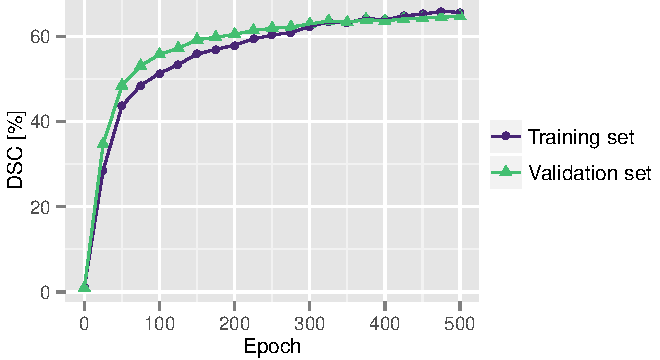
\includegraphics[width=0.7\textwidth]{figures/tmi/ems_progress}
\caption[Improvement in the mean DSC computed on the training and test sets
during training]{Improvement in the mean DSC computed on the training and test
sets during training. Only small improvements can be observed after 400 epochs.}
\label{fig:epochs}
\end{figure}

To determine an effective sensitivity ratio, we measured the performance on the
validation set over a range of values. For each choice of ratio, we binarized
the segmentations using a threshold that maximized the DSC on the training set.
\ref{fig:ratio} shows a set of \gls{roc} curves for different choices of the
sensitivity ratio ranging from 0.01 to 0.10 and the corresponding optimal
thresholds. The plots illustrate our findings that our method is not sensitive
to the choice of the sensitivity ratio, which mostly affects the optimal
threshold. We chose a fixed sensitivity ratio of 0.02 for all our experiments.

\begin{figure}[tb]
\centering
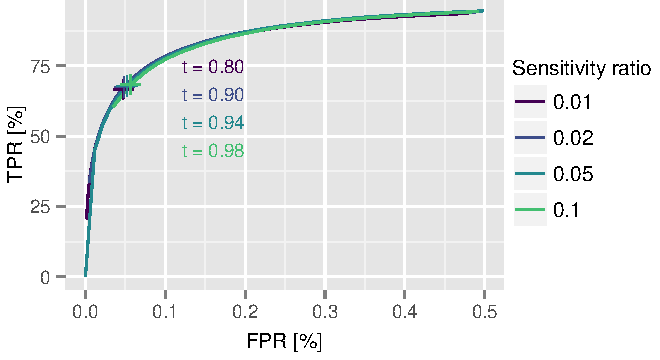
\includegraphics[width=0.7\textwidth]{figures/tmi/roc2}
\caption[ROC curves for different sensitivity ratios $r$]{ROC curves for
different sensitivity ratios $r$. A `$+$' marks the TPR and FPR of the optimal
threshold. Varying the value of $r$ results in almost identical ROC curves and
only causes a change of the optimal threshold $t$, which shows the robustness of
our method with respect to the sensitivity ratio.}
\label{fig:ratio}
\end{figure}


\subsection[Impact of the training set size on the segmentation
performance]{Impact of the Training Set Size on the Segmentation Performance}

To evaluate the impact of the training set size on the segmentation performance,
we trained a CEN with 3 layers on the first in-house data set with varying
number of training samples and calculated the mean DSC on the training and test
sets as illustrated in \ref{fig:bioms}. For small training sets, there is a
large difference between the DSCs on the training and test sets, which indicates
that the training set is too small to learn a representative set of features. At
around 100 samples, the model becomes stable in terms of test performance and
the small differences between training and test DSCs, indicating that
overfitting of the training data is no longer occurring. With 100 training
subjects, our method achieves a mean DSC on the test set of
\SI{57.38}{\percent}.

% , which shows
% that the segmentation accuracy can be greatly improved compared to the results
% on the challenge data set, when a representative training set is available.

\begin{figure}[tb]
\centering
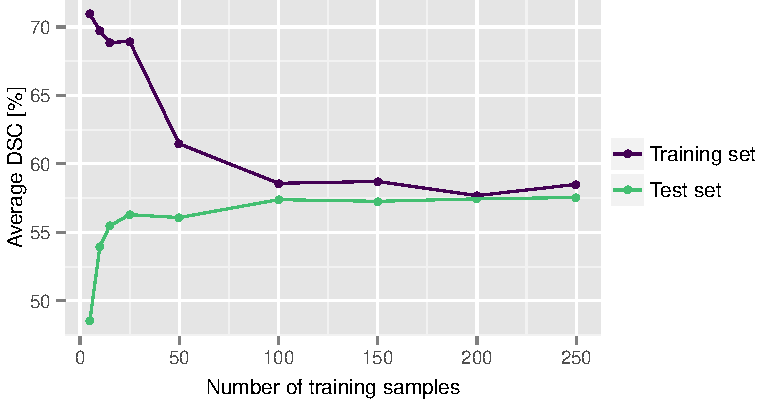
\includegraphics[width=0.8\textwidth]{figures/train_count}
\caption[Comparison of DSC scores calculated on the training and test sets for
varying numbers of training samples]{Comparison of DSC scores calculated on the
training and test sets for varying numbers of training samples. At around 100
samples, the model becomes stable in terms of test performance and the small
difference between training and test DSCs, indicating that overfitting of the
training data no longer occurs.}
\label{fig:bioms}
\end{figure}

\subsection[Comparison on public data sets]{Comparison on Public Data Sets}

% TODO: Can you add some comments on the challenges for human
% observers in the ground truth segmentation? If you have information about
% intra- and inter-rater variability please add these here and discuss these.
% I might be able to do this. I need to see if I have ground truth information
% from both raters or only of one.

To allow for a direct comparison with a large number of state-of-the-art
methods, we evaluated our method on the MICCAI 2008 MS lesion segmentation
challenge \citep{styner20083d} and the ISBI 2015 longitudinal MS lesion
segmentation challenge. As shown in the previous section, approximately 100
images are required to train the 3-layer CEN without overfitting and we expect
the required number of images to be even higher when adding more layers.
Due to the relatively small size of the training data sets provided by the two
challenges, we used a CEN with only three layers on these data sets to reduce
the risk of overfitting. The parameters of the models are summarized in
\ref{tab:archchallenge}.

\begin{table}[tb]
\caption[Parameters of the 3-layer CEN for the evaluation on the challenge data
sets]{Parameters of the 3-layer CEN for the evaluation on the challenge data
sets. The number of input channels $c$ is 3 for the MICCAI challenge and 4 for
the ISBI challenge.}
\label{tab:archchallenge}
\centering
\begin{tabular}{lccr}
\toprule
Layer type & Kernel Size & \#Filters & \multicolumn{1}{c}{Number of Units} \\
\midrule
Input & --- & --- & $164\times 206\times 156\times c$\phantom{0} \\
Convolutional & $9\times 9\times 9\times c$\phantom{0} & 32 &
\num{156x198x148x32} \\
Deconvolutional & \num{9x9x9x32} & 1 & \num{164x206x156x1}\phantom{0} \\
\bottomrule
\end{tabular}
\end{table}

\begin{figure}[tb]
\centering
\small
\def\MRIwidth{0.15\textwidth}

\begin{tikzpicture} 
\tikzstyle{leftlabel}=[rotate=90, align=center,overlay,above]

\matrix [matrix of nodes, nodes={anchor=center, inner sep=1pt}] {
        &[4pt] FLAIR & T1w & T2w & Ground truth & Our method \\[4pt]
\node[leftlabel] {CHB\,07\\(DSC\,=\,\SI{60.58}{\percent})}; &
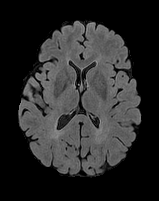
\includegraphics[width=\MRIwidth]{figures/MICCAI2015_CHB07-FLAIR-s88} &
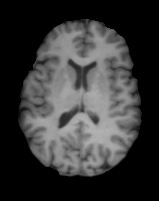
\includegraphics[width=\MRIwidth]{figures/MICCAI2015_CHB07-T1w-s88} &
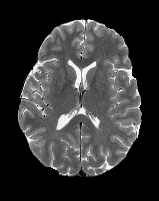
\includegraphics[width=\MRIwidth]{figures/MICCAI2015_CHB07-T2w-s88} &
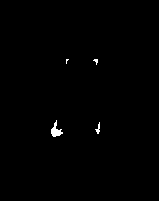
\includegraphics[width=\MRIwidth]{figures/MICCAI2015_CHB07-gold-s88} &
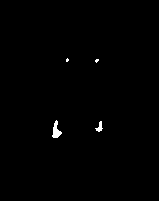
\includegraphics[width=\MRIwidth]{figures/MICCAI2015_CHB07-pred-s88} \\
\node[leftlabel] {CHB\,04\\(DSC\,=\,\SI{61.37}{\percent})}; &
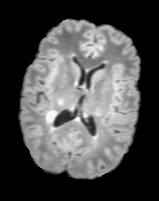
\includegraphics[width=\MRIwidth]{figures/MICCAI2015_CHB04-FLAIR-s85} &
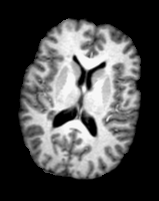
\includegraphics[width=\MRIwidth]{figures/MICCAI2015_CHB04-T1w-s85} &
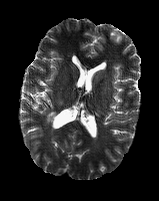
\includegraphics[width=\MRIwidth]{figures/MICCAI2015_CHB04-T2w-s85} &
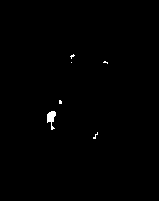
\includegraphics[width=\MRIwidth]{figures/MICCAI2015_CHB04-gold-s85} &

\includegraphics[width=\MRIwidth]{figures/MICCAI2015_CHB04-pred-s85} \\
\node[leftlabel] {UNC\,09\\(DSC\,=\,\SI{9.01}{\percent})}; &
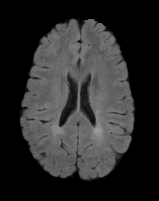
\includegraphics[width=\MRIwidth]{figures/MICCAI2015_UNC09-FLAIR-s89} &
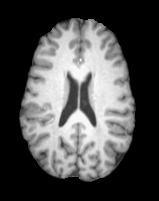
\includegraphics[width=\MRIwidth]{figures/MICCAI2015_UNC09-T1w-s89} &
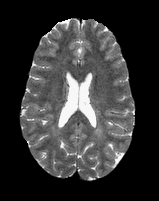
\includegraphics[width=\MRIwidth]{figures/MICCAI2015_UNC09-T2w-s89} &

\includegraphics[width=\MRIwidth]{figures/MICCAI2015_UNC09-gold-s89} &
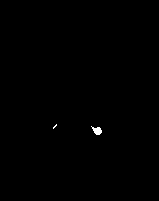
\includegraphics[width=\MRIwidth]{figures/MICCAI2015_UNC09-pred-s89} \\
};
\end{tikzpicture}

\caption[Example segmentations of our method for three different subjects from
the MICCAI challenge data set]{Example segmentations of our method for three
different subjects from the MICCAI challenge data set. Our method performed well
and consistently despite the large contrast differences seen between the first
two rows. In the third row, our method also segmented lesions that have similar
contrast, but these regions had not been identified as lesions by the manual
rater, which highlights the difficulty in distinguishing focal lesions from
diffuse damage, even for experts.}

\label{fig:segmentation}
\end{figure}

\subsubsection{MICCAI 2008 MS Lesion Segmentation Challenge}

In a first experiment, we evaluated the performance of our method using 5-fold
cross-validation on the training set of the MICCAI challenge.
\ref{fig:segmentation} shows a comparison of lesion masks produced by our method
with the ground truth for three subjects. The first two rows show the FLAIR,
T1w, T2w, ground truth segmentations, and predicted segmentations of two
subjects with a DSC of \SI{60.58}{\percent} and \SI{61.37}{\percent}. Despite
the large contrast differences between the two subjects, our method performed
well and consistently, which indicates that our model was able to learn features
that are robust to a large range of intensity variations. The last row shows a
subject with a DSC of \SI{9.01}{\percent}, one of the lowest DSC scores from the
data set. Our method segmented lesions that have similar contrast to the other
two subjects, but these regions were not classified as lesions by the manual
rater. This highlights the difficulty of manual lesion segmentation, as the
difference between diffuse white matter pathology and focal lesions is often
indistinct.

A quantitative comparison of our method with other state-of-the-art
methods is summarized in \ref{tab:state}. Our method outperforms the winning
method \citep{souplet2008} of the MS lesion segmentation challenge 2008 and the
currently best unsupervised method reported on that data set \citep{weiss2013}
in terms of mean TPR and PPV. Our method performs comparably to a current method
\citep{geremia2010,geremia2011} that uses a carefully designed set of features
specifically designed for lesion segmentation, despite our method having learned its features
solely from a relatively small training set.

\begin{table}[tb]
\def\tabspace{12pt}

\caption[Comparison of our method with state-of-the-art lesion segmentation
methods]{Comparison of our method with state-of-the-art lesion segmentation
methods in terms of mean TPR, PPV, and DSC on the training set of the MICCAI
2008 lesion segmentation challenge. Our method performs comparably to the best
methods reported on the MS lesion segmentation challenge data set.}

\label{tab:state}
\centering
\begin{tabular}{l%
@{\hspace{\tabspace}}S[table-format=2.2]
@{\hspace{\tabspace}}S[table-format=2.2]
@{\hspace{\tabspace}}S[table-format=2.2]
}
\toprule
Method & {TPR} & {PPV} & {DSC} \\ 
\midrule
\citet{souplet2008} & 20.65 & 30.00 & {---} \\ 
\citet{weiss2013} & 33.00 & 36.85 & 29.05 \\ 
\citet{geremia2010} & 39.85 & 40.35 & {---}  \\
Our method & 39.71 & 41.38 & 35.52 \\
\bottomrule
\end{tabular}
\end{table}

A comparison of our method with other state-of-the-art methods evaluated on the
test set of the MICCAI challenge is summarized in \ref{tab:miccai}. Our method
ranked 6th (2nd if only considering methods with only one submission, i.e.,
without subsequent parameter-tuning and adjustments) out of 52 entries submitted
to the challenge, outperforming the recent SLS by \citet{roura2015}, and popular
methods such as the random forest approach by \citet{geremia2010}, and
Lesion-TOADS by \citet{shiee2010}, but not as well as the patch-based
segmentation approach by \citet{guizard2015}, or the \gls{mops} approach by
\citet{tomas2015}, which used additional images to build the intensity model of
a healthy population. This is a very promising result for the first submission
of our method given the simplicity of the model and the small training set size.

\begin{table}[tb]
\sisetup{
  round-mode = places,
  round-precision = 2}%
\caption[Selected methods out of the 52 entries submitted for evaluation to the
MICCAI 2008 MS lesion segmentation challenge]{Selected methods out of the 52
entries submitted for evaluation to the MICCAI 2008 MS lesion segmentation
challenge. Columns LTPR, LFPR, and VD show the average computed from the two
raters in percent. Challenge results last updated: Dec 15, 2015.}
\label{tab:miccai}
\centering
\begin{tabular}{clS[table-format=2.2]
S[table-format=2.1,round-precision=1]
S[table-format=2.1,round-precision=1]
S[table-format=2.1,round-precision=1]}
\toprule
Rank & Method & {Score} & {LTPR} & {LFPR} & {VD} \\
\midrule
$1,3,9$  & \citet{jesson2015} & 86.9386 & 48.70 & 28.25 & 80.15 \\
2  & \citet{guizard2015}   & 86.1071 & 49.85 & 42.75 & 48.80 \\
$4,20,26$  & \citet{tomas2015} & 84.464 & 46.9 & 44.6 &
45.60 \\
$5,7$ & \citet{jerman2015}        & 84.1555 & 65.15 & 63.75 & 77.45 \\
6  & Our method    & 84.0743 & 51.55 & 51.25 & 57.75 \\
11 & \citet{roura2015} & 82.3442 & 50.15 & 41.85 & 111.60 \\
13 & \citet{geremia2010}     & 82.0691 & 55.1 & 74.1 & 48.90 \\
24 & \citet{shiee2010} & 79.8975 & 52.4 & 72.7 & 74.45 \\
\bottomrule
\end{tabular}
\end{table}

\subsubsection{ISBI 2015 Longitudinal MS Lesion Segmentation Challenge}

In addition, we evaluated our method on the 21 publicly available labeled cases
from the ISBI 2015 longitudinal MS lesion segmentation challenge. The challenge
organizers have only released the names of the top three teams, only two of
which have published a summary of their mean DSC, LTPR, and LFPR scores for both
raters to allow for a direct comparison. Following the evaluation protocol of
the second \citep{jesson2015} and third \citep{maier2015} place methods, we
trained our model using leave-one-subject-out cross-validation on the training
images and compared our results to the segmentations provided by both raters.
\ref{tab:isbi} summarizes the performance of our method, the two other
methods for comparison, and the performance of the two raters when compared
against each other. Compared to the second and third place methods, our method
was more sensitive and produced significantly higher LTPR scores, but also had
more false positives, which resulted in slightly lower but still comparable DSC
scores. This is again a promising result on a public data set.

\begin{table}[tb]
\caption[Comparison of our method with the second and third ranked methods from
the ISBI MS lesion segmentation challenge]{Comparison of our method with the
second and third ranked methods from the ISBI MS lesion segmentation challenge.
The evaluation was performed on the training set using leave-one-subject-out
cross-validation. GT1 and GT2 denote that the model was trained with the
segmentations provided by the first and second rater as the ground truth,
respectively.}
\label{tab:isbi}
\centering
\begin{tabular}{lcccccc}
\toprule
Method &
\multicolumn{3}{c}{Rater 1} &
\multicolumn{3}{c}{Rater 2} \\
& DSC & LTPR & LFPR & DSC & LTPR & LFPR \\
\midrule
Rater 1 & --- & --- & --- & 73.2 & 64.5 & 17.4 \\
Rater 2 & 73.2 & 82.6 & 35.5 & --- & --- & --- \\
\citet{jesson2015} &  70.4 & 61.1 & 13.5 & 68.1 & 50.1 & 12.7 \\
\citet{maier2015} (GT1) & 70 & 53 & 48 & 65 & 37 & 44 \\
\citet{maier2015} (GT2) & 70 & 55 & 48 & 65 & 38 & 43 \\
Our method (GT1) & 68.4 & 74.5 & 54.5 & 64.4 & 63.0 & 52.8 \\
Our method (GT2) & 68.3 & 78.3 & 64.5 & 65.8 & 69.3 & 61.9 \\
\bottomrule
\end{tabular}
\end{table}

\subsection[Comparison of network architectures, input modalities, and publicly
available methods on clinical trial data]{Comparison of Network Architectures,
Input Modalities, and Publicly Available Methods on Clinical Trial Data}

\begin{table}[tb]
\caption{Parameters of the 3-layer CEN used on the clinical trial data set.}
\label{tab:arch3}
\centering
\begin{tabular}{lccr}
\toprule
Layer type & Kernel Size & \#Filters & \multicolumn{1}{c}{Number of Units} \\
\midrule
Input & --- & --- & \num{164x206x52x2}\phantom{0} \\
Convolutional & \num{9x9x5x2} & 32 & \num{156x198x48x32} \\
Deconvolutional & \num{9x9x5x32} & 1 & \num{164x206x52x1}\phantom{0} \\
\bottomrule
\end{tabular}
\end{table}

\subsubsection[Quantitative comparison]{Quantitative Comparison}

To determine the effect of network architectures, we compared the segmentation
performance of three different networks using T1w and FLAIR MRIs.
Specifically, we trained a 3-layer CEN and two 7-layer CENs, one with shortcut
connections and one without. To investigate the effect of different input image
types, we additionally trained two 7-layer CEN-s on the modalities used by EMS
(T1w, T2w, PDw) and all four modalities (T1w, T2w, PDw, FLAIR). The parameters
of the networks are given in \ref{tab:arch3} and \ref{tab:arch7}. To
roughly compensate for the anisotropic voxel size of the input images, we chose
an anisotropic filter size of \num{9x9x5}. In addition, we ran the five
competing methods discussed in \ref{sec:othermethods} with Lesion-TOADS, SLS,
and the two LST methods using the T1w and FLAIR images, and EMS using three
(T1w, T2w, PDw) and all four modalities in separate tests. A comparison of the
segmentation accuracy of the trained networks and competing methods is
summarized in \ref{tab:results1}.

\begin{table}[tb]
\caption{Parameters of the 7-layer CEN-s used on the clinical trial data set.}
\label{tab:arch7}
\centering
\begin{tabular}{lccr}
\toprule
Layer type & Kernel Size & \#Filters & \multicolumn{1}{c}{Number of Units} \\
\midrule
Input & --- & --- & \num{164x206x52x2}\phantom{0} \\
Convolutional & \num{9x9x5x2} & 32 & \num{156x198x48x32} \\
{Average Pooling} & \num{2x2x2} & --- & \num{78x99x24x32} \\
{Convolutional} & \num{9x10x5x32} & 32 & \num{70x90x20x32} \\
{Deconvolutional} & \num{9x10x5x32} & 32 & \num{78x99x24x32} \\
{Unpooling }& \num{2x2x2} & --- & \num{156x198x48x32} \\
{Deconvolutional }& \num{9x9x5x32} & 1 & \num{164x206x52x1}\phantom{0} \\
\bottomrule
\end{tabular}
\end{table}

\begin{table}[tb]
\caption[Comparison of the segmentation accuracy of different CEN models, other
methods, and input modalities.]{Comparison of the segmentation accuracy of
different CEN models, other methods, and input modalities. The table shows the
mean of the Dice similarity coefficient (DSC), lesion true positive rate (LTPR),
and lesion false positive rate (LFPR). Because the volume difference (VD) is not
limited to the interval $[0, 100]$, a single outlier can heavily affect the
calculation of the mean. We therefore excluded outliers before calculating the
mean of the VD for all methods using the box plot criterion.}
\centering
\small
\label{tab:results1}
\begin{tabular}{lcccc}
\toprule
Method & DSC [\%] & LTPR [\%] & LFPR [\%] & VD [\%] \\
\midrule
\multicolumn{5}{c}{\textit{Input modalities: T1w and FLAIR}} \\
\midrule
3-layer CEN & 49.24 & 57.33 & 61.39 & 43.45 \\
7-layer CEN & 52.07 & 43.88 & 29.06 & 37.01 \\ 
7-layer CEN-s & 55.76 & 54.55 & 38.64 & 36.30 \\[0.2em]
Lesion-TOADS \citep{shiee2010} & 40.04 & 56.56 & 82.90 & 49.36 \\ 
SLS \citep{roura2015}  & 43.20 &  56.80 & 50.80 & 12.30 \\
LST-LGA \citep{schmidt2012} & 46.64 & 37.50 & 38.06 & 36.77 \\
LST-LPA \citep{schmidt2012} & 46.07 & 48.02 & 52.94 & 41.62 \\
\midrule
\multicolumn{5}{c}{\textit{Input modalities: T1w, T2w, and PDw}} \\
\midrule
7-layer CEN-s & 61.18 & 52.00 & 36.68 & 29.38 \\
EMS \citep{vanleemput2001} & 42.94 & 44.80 & 76.58 & 49.29 \\
\midrule
\multicolumn{5}{c}{\textit{Input modalities: T1w, T2w, FLAIR, and PDw}} \\
\midrule
7-layer CEN-s & 63.83 & 62.49 & 36.10 & 32.89 \\
EMS \citep{vanleemput2001} & 39.70 & 49.08 & 85.01 & 34.51 \\
\bottomrule
\end{tabular}
\end{table}

All CEN architectures performed significantly better than all other methods
regardless of the input modalities, with LST-LGA being the closest in overall
segmentation accuracy. Comparing CEN to LST-LGA, the improvements in the mean
DSC scores ranged from 3 \gls{pp} for the 3-layer CEN to 17\,pp
for the 7-layer CEN with shortcut trained on all four modalities. The improved
segmentation performance was mostly due to an increase in lesion sensitivity.
LST-LGA achieved a mean lesion TPR of \SI{37.50}{\percent}, compared to
\SI{54.55}{\percent} produced by the CEN with shortcut when trained on the same
modalities, and \SI{62.49}{\percent} when trained on all four modalities, while
achieving a comparable number of lesion false positives. The mean lesion FPRs
and mean volume differences of LST-LGA and the 7-layer CEN-s were very close,
when trained on the same modalities, and the CEN-s further reduced its FPR when
trained on more modalities.

This experiment also showed that increasing the depth of the CEN and adding the
shortcut connections both improve the segmentation accuracy. Increasing the
depth of the CEN from three layers to seven layers improved the mean DSC by
3\,pp. The improvement was confirmed to be statistically significant using a
one-sided paired $t$-test ($p$-value of \num{1.3e-5}). Adding a shortcut to the
network further improved the segmentation accuracy as measured by the DSC by
3\,pp. A second one-sided paired $t$-test was performed to confirm the
statistical significance of the improvement with a $p$-value of less than
\num{1e-10}.

\subsubsection{Qualitative Comparison of Network Architectures}

The impact of increasing the depth of the network on the segmentation
performance of very large lesions is illustrated in \ref{fig:large}, where the
true positive, false negative, and false positive voxels are highlighted in
green, yellow, and red, respectively. The receptive field of the 3-layer CEN has
a size of only \num{17x17x9} voxels, which reduces its ability to identify very
large lesions marked by two white circles. In contrast, the 7-layer CEN has a
receptive field size of \num{49x53x26} voxels, which allows it to learn features
that can capture much larger lesions. Consequently, the 7-layer CEN, with and
without shortcut, is able to learn a feature set that captures large lesions
much better than the 3-layer CEN, which results in an improved segmentation.
However, increasing the depth of the network without adding shortcut connections
reduces the network's sensitivity to very small lesions as illustrated in
\ref{fig:small}. In this example, the 3-layer CEN was able to detect three small
lesions, indicated by the white circles, which were missed by the 7-layer CEN.
Adding shortcut connections enables our model to learn a feature set that spans
a wider range of lesion sizes, which increases the sensitivity to small lesions
and, hence, allows the 7-layer \mbox{CEN-s} to detect all three small lesions
(highlighted by the white circles), while still being able to segment large
lesions.

\begin{figure}[p]
\centering
\begin{tikzpicture}[node distance=3.2cm and 0.3\textwidth,
  font=\small, on grid]
\node[inner sep=0] (image1) {
  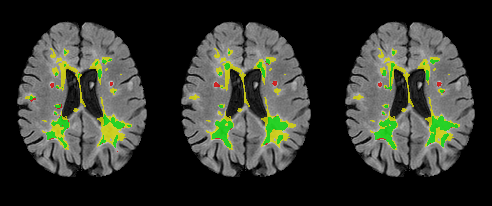
\includegraphics[width=0.9\textwidth]{figures/tmi/p50s35_large_lesions}
};
\node[above=of image1] (l7) {7-layer CEN};
\node[left=of l7] {3-layer CEN};
\node[right=of l7] {7-layer CEN-s};

\begin{scope}[xshift=0.3\textwidth,scale=1.6]
\draw[white,thick] (-12pt,-15pt) circle (9pt);
\draw[white,thick] (15pt,-15pt) circle (10pt);
\end{scope}
\begin{scope}[xshift=-0.3\textwidth,scale=1.6]
\draw[white,thick] (-12pt,-15pt) circle (9pt);
\draw[white,thick] (15pt,-15pt) circle (10pt);
\end{scope}
\begin{scope}[scale=1.6]
\draw[white,thick] (-12pt,-15pt) circle (9pt);
\draw[white,thick] (15pt,-15pt) circle (10pt);
\end{scope}
\end{tikzpicture}
\caption[Impact of increasing the depth of the network on the segmentation
performance of very large lesions]{Impact of increasing the depth of the network on the segmentation
performance of very large lesions. The true positive, false negative, and false
positive voxels are highlighted in green, yellow, and red, respectively. The
7-layer CEN, with and without shortcut, is able to segment large lesions much
better than the 3-layer CEN due to the increased size of the receptive field.
This figure is best viewed in colour.}
\label{fig:large}
\end{figure}

\begin{figure}[p]
\centering
\begin{tikzpicture}[node distance=3.2cm and 0.3\textwidth,
  font=\small, on grid,spy using outlines={circle, connect spies}]
  
\node[inner sep=0] (image1) {
  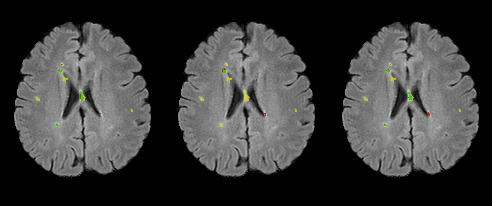
\includegraphics[width=0.9\textwidth]{figures/tmi/p25s35_small_lesions}
};
\node[above=of image1] (l7) {7-layer CEN};
\node[left=of l7] {3-layer CEN};
\node[right=of l7] {7-layer CEN-s};

\begin{scope}[xshift=0.3\textwidth]
\coordinate (on1) at (-15.2pt,30.5pt);
\coordinate (in1) at (-32pt,54pt);
\spy[white,thick,size=40pt,magnification=6] on (on1) in node[overlay] at (in1);

\coordinate (on2) at (0pt,5.5pt);
\coordinate (in2) at (28pt, 50pt);
\spy[white,thick, size=54pt, magnification=3.5, xshift=0.3\textwidth] on
(on2) in node[overlay] at (in2);

\coordinate (on3) at (-19.5pt,-18pt);
\coordinate (in3) at (10pt,-52pt);
\spy[white,thick, size=40pt, magnification=6, xshift=0.3\textwidth] on
(on3) in node[overlay] at (in3);
\end{scope}

\begin{scope}[xshift=-0.3\textwidth]
\coordinate (on4) at (-15.2pt,30.5pt);
\coordinate (in4) at (-32pt,54pt);
\spy[white,thick,size=40pt,magnification=6] on (on4) in node[overlay] at (in4);

\coordinate (on5) at (0pt,5.5pt);
\coordinate (in5) at (28pt, 50pt);
\spy[white,thick, size=54pt, magnification=3.5, xshift=0.3\textwidth] on
(on5) in node[overlay] at (in5);

\coordinate (on6) at (-19.5pt,-18pt);
\coordinate (in6) at (10pt,-52pt);
\spy[white,thick, size=40pt, magnification=6, xshift=0.3\textwidth] on
(on6) in node[overlay] at (in6);
\end{scope}

\spy[white,thick, size=40pt, magnification=6] on (-15.2pt,30.5pt)
in node[overlay] at (-32pt,54pt);
\spy[white,thick, size=54pt, magnification=3.5] on (0pt,5.5pt)
in node[overlay] at (28pt, 50pt);
\spy[white,thick, size=40pt, magnification=6] on (-19.5pt,-18pt)
in node[overlay] at (10pt,-52pt);
\end{tikzpicture}

\caption[Comparison of segmentation performance of different CEN architectures
for small lesions]{Comparison of segmentation performance of different CEN architectures
for small lesions. The white circles indicate lesions that were detected by the
3-layer CEN and the 7-layer CEN, but only with shortcut. Increasing the network
depth decreases the sensitivity to small lesions, but the addition of a
shortcut allows the network to regain this ability, while still being able to
detect large lesions (see \ref{fig:large}). This figure is best viewed in
colour.}
\label{fig:small}
\end{figure}

\subsection[Comparison for different lesion sizes]{Comparison for Different
Lesion Sizes}

To examine the effect of lesion size on segmentation performance, we stratified
the test set into five groups based on their mean reference lesion size as
summarized in \ref{tab:groups}. A comparison of segmentation accuracy and lesion
detection measures of a 7-layer CEN-s trained on different input modalities and
the best performing competing method LST-LGA for different lesion sizes is
illustrated in \ref{fig:sizecomp}. The 7-layer CEN-s outperformed LST-LGA for
all lesions sizes except for very large lesions when trained on T1w and FLAIR
MRIs. The advantage extended to all lesion sizes when the \mbox{CEN-s} was
trained on all four modalities, which could not be done for LST-LGA.
The differences were larger for smaller lesions, which are generally more
challenging to segment for all methods. The differences between the two
approaches were due to a higher sensitivity to lesions as measured by the LTPR,
especially for smaller lesions, while the number of false positives was
approximately the same for all lesion sizes.

\begin{table}[tb]
\caption{Lesion size groups as used for the detailed analysis.}
\label{tab:groups}
\centering
\begin{tabular}{lccc}
\toprule
Group & Mean lesion size [\si{\cubic\milli\metre}] & \#Samples & Lesion
load [\si{\cubic\milli\metre}] \\
\midrule
Very small & $[0,70]$ & 6 & \num{1457+-1492} \\
Small      & $(70,140]$ & 24 & \num{4298+-2683} \\
Medium & $(140,280]$ & 24 & \num{12620+-9991} \\
Large & $(280,500]$ & 14 & \num{13872+-5814} \\
Very large & $> 500$ & 9 & \num{35238+-27531} \\
\bottomrule
\end{tabular}
\end{table}

\begin{figure}
\centering
%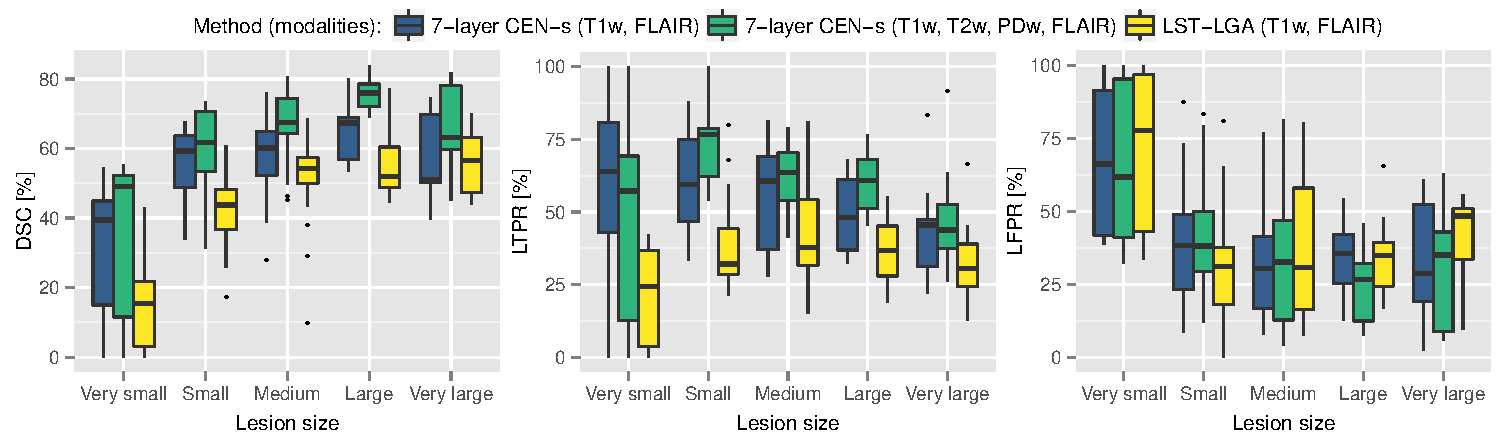
\includegraphics[width=\textwidth]{figures/tmi/cen_vs_LGA_size}
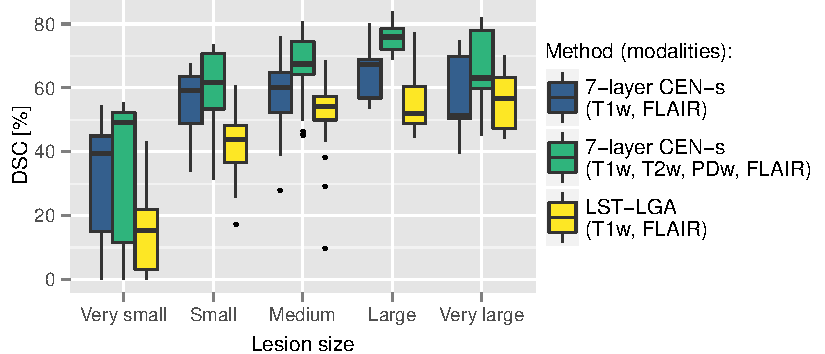
\includegraphics[width=0.78\textwidth]{figures/tmi/dsc}
\\[1em]
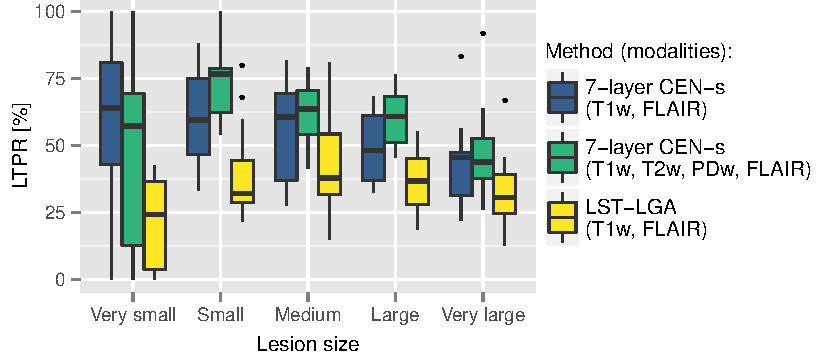
\includegraphics[width=0.78\textwidth]{figures/tmi/tpr}
\\[1em]
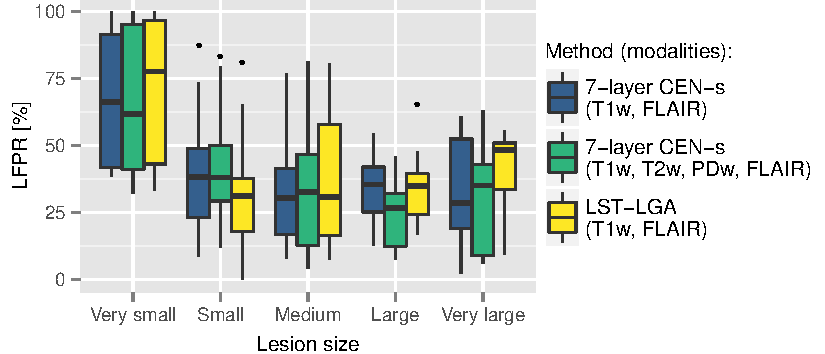
\includegraphics[width=0.78\textwidth]{figures/tmi/fpr}

\caption[Comparison of segmentation accuracy and lesion detection measures of a
7-layer CEN-s and LST-LGA for different lesion sizes]{Comparison of segmentation
accuracy and lesion detection measures of a 7-layer CEN-s trained on different
input modalities and the best performing competing method LST-LGA for different
lesion sizes. The 7-layer CEN-s outperforms LST-LGA for all lesions sizes except
for very large lesions when trained on T1w and FLAIR MRIs, and for all lesion
sizes when trained on all four modalities, due to a higher sensitivity to
lesions, while producing approximately the same number of false positives.
Outliers are denoted by black dots.}

\label{fig:sizecomp}
\end{figure}

\section{Discussion}

The automatic segmentation of MS lesions is a very challenging task due to the
large variability in lesion size, shape, intensity, and location, as well as the
large variability of imaging contrasts produced by different scanners used in
multi-centre studies. Most unsupervised methods model lesions as an outlier
class or a separate cluster in a subject-specific model, which makes them
inherently robust to inter-subject and inter-scanner variability. However,
outliers are often not specific to lesions and can also be caused by intensity
inhomogeneities, partial volume, imaging artifacts, and small anatomical
structures such as blood vessels, which leads to the generation of false
positives. On the other hand, supervised methods can learn to discriminate
between lesion and non-lesion tissue, but are more sensitive to the variability
in lesion appearance and different contrasts produced by different scanners. To
overcome those challenges, supervised methods require large data sets that span
the variability in lesion appearance and careful preprocessing to match the
imaging contrast of new images with those of the training set. Library-based
approaches have shown great promise for the segmentation of MS lesions, but do
not scale well to very large data sets due to the large amount of memory
required to store comprehensive sample libraries and the time required to scan
such libraries for matching patches. On the other hand, parametric deep learning
models such as convolutional neural networks scale much better to large training
sets, because the size required to store the model is independent of the
training set size, and the operations required for training and inference are
inherently parallelizable, which allows them to take advantage of very fast
GPU-accelerated computing hardware. Furthermore, the combination of many
nonlinear processing units allows them to learn features that are robust under
large variability, which is crucial for the segmentation of MS lesions.

Convolutional neural networks were originally designed to classify entire images
and designing networks that can segment images remains an important research
topic. Early approaches have formulated the segmentation problem as a patch-wise
classification problem, which allows them to directly use established
classification network architectures for image segmentation.
However, a major limitation of patch-based deep learning approaches is the time
required for training and inference. Fully convolutional networks can perform
the segmentation much more efficiently, but generally lack the precision to
perform voxel-accurate segmentation and cannot handle unbalanced classes.

To overcome these challenges, we have presented a new method for the automatic
segmentation of MS lesions based on deep convolutional encoder networks with
shortcut connections. The joint training of the feature extraction and
prediction pathways allows for the automatic learning of features at different
scales that are tuned for a given combination of image types and segmentation
task. Shortcuts between the two pathways allow high- and low-level features to
be leveraged at the same time for more consistent performance across scales. In
addition, we have proposed a new objective function based on the combination of
sensitivity and specificity, which makes the objective function inherently
robust to unbalanced classes such as MS lesions, which typically comprise less
than \SI{1}{\percent} of all image voxels. We have evaluated our method on two
publicly available data sets and a large data set from an MS clinical trial,
with the results showing that our method performs comparably to the best
state-of-the-art methods, even for relatively small training set sizes. We have
also shown that when a suitably large training set is available, our method is
able to segment MS more accurately than widely-used competing methods such as
EMS, LST-LGA, SLS, and Lesion-TOADS. The substantial gains in accuracy were
mostly due to an increase in lesion sensitivity, especially for small lesions.
Overall, our proposed CEN with shortcut connections performed consistently well
over a wide range of lesion sizes.

Our segmentation framework is very flexible and can be easily extended. One such
extension could be to incorporate prior knowledge about the tissue type of each
non-lesion voxel into the segmentation procedure. The probabilities of each
tissue class could be precomputed by a standard segmentation method, after which
they can be added as an additional channel to the input units of the CEN, which
would allow the CEN to take advantage of intensity information from different
modalities and prior knowledge about each tissue class to carry out the
segmentation. In addition, our method can be applied to other segmentation
tasks. Although we have only focused on the segmentation of MS lesions in this
paper, our method does not make any assumptions specific to MS lesion
segmentation. The features required to carry out the segmentation are solely
learned from training data, which allows our method to be used to segment
different types of pathology or anatomy when a suitable training set is
available.
